\section{ผลลัพธ์ประสิทธิภาพการทำงานระหว่าง HAPS และ Terrestrial Networks}
สาเหตุของสัญญาณรบกวนนั้น เกิดจากข้อจำกัดปริมาณการส่งข้อมูลใน 1 ชุดคำสั่ง(Protocol)
HAPS กระจายสัญญาณครอบคลุมในพื้นที่วงกว้าง จึงทำให้ไม่สามารถแยกแยะความถี่ในแต่ละคลื่นสัญญาณได้
การสื่อสารระหว่างสัญญาณจาก HAPS ไปยังสถานีภาคพื้นดินหลัก(Base Station - BS)
และอุปกรณ์รับสัญญาณของผู้ใช้งานทั่วไป เช่น Smartphone(User Equipment - UE) 

\begin{figure}[h]
\centering
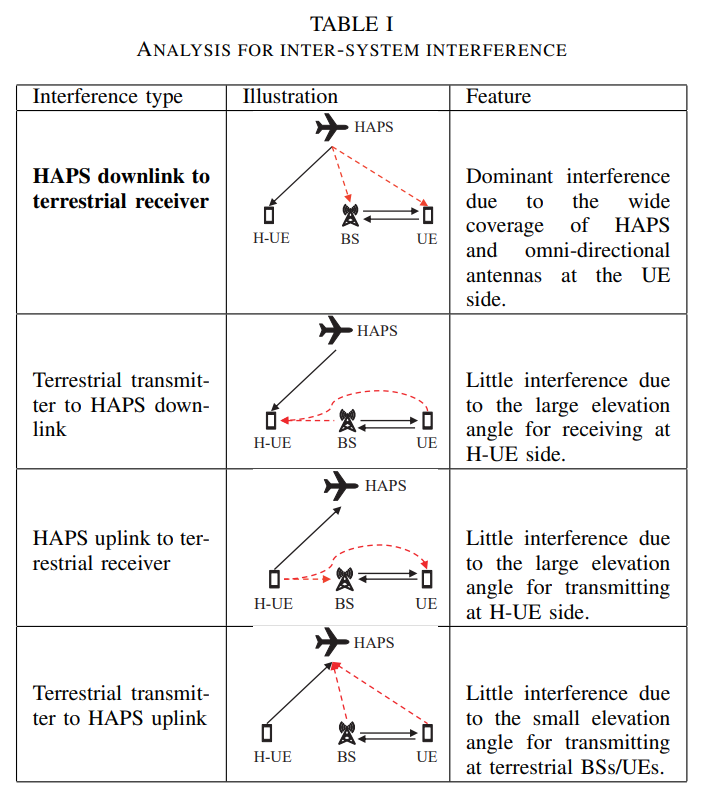
\includegraphics[width=0.3\textwidth]{HAPS-with-TN.png}
\end{figure}

\centering รูปที่ 1 : Analysis for Inter-System Interference 
\begin{itemize}
    \item Type 1 - เกิดสัญญาณรบกวนเป็นหลักที่ฝั่ง UE
    \item Type 2 - เกิดสัญญาณรบกวนเล็กน้อยที่ฝั่ง H-UE
    \item Type 3 - สัญญาณ Uplink เกิดสัญญาณรบกวนเล็กน้อยที่ฝั่ง H-UE แสดงให้เห็นว่าการปรับทิศทางส่งสัญญาณส่งผล
    ต่อการลดสัญญาณรบกวน
    \item Type 4 - การส่งสัญญาณจากสถานีหลัก(Base Station - BS) ไป HAPS Uplink
\end{itemize}

ผลการทดลองทั้ง 4 Type สรุปได้ว่าสัญญาณที่ส่งจากสถานีหลักไปยัง HAPS ด้วยการปรับมุมและทิศทางสามารถช่วยลดโอกาสที่จะเกิดสัญญาณรบกวนและลดปริมาณทรัพยากรที่ใช้ และประเมินผลออกมาเป็นกราฟดังนี้

\begin{figure}[h]
\centering
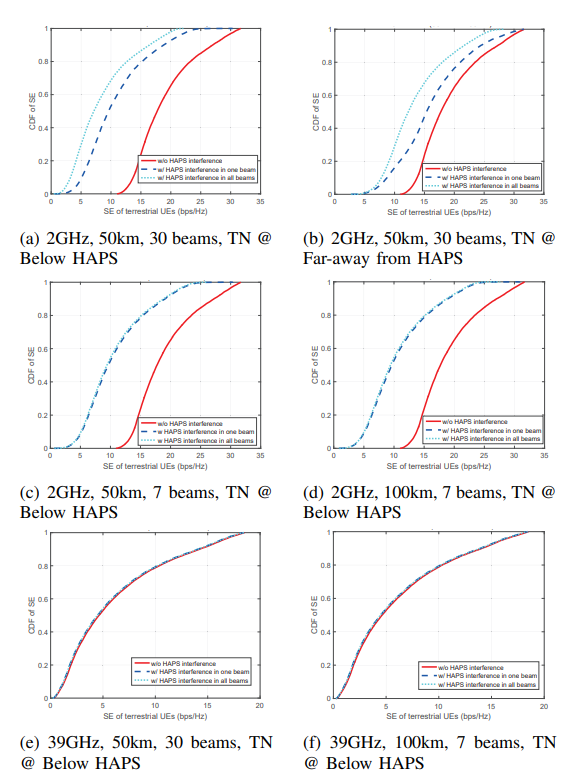
\includegraphics[width=0.3\textwidth]{HAPS-comapare-downlink.png}
\end{figure}

\centering รูปที่ 2 : Downlink SE performance in terrestrial network (TN) with or without the interference 
from HAPS downlink.
\\
กราฟแสดงถึงผลที่เกิดจากสัญญาณรบกวนจาก HAPS ไปยังสถานีภาคพื้นดิน(TN) และอุปกรณ์ของผู้ใช้(UE)
ในความถี่และรัศมีครอบคลุมที่แตกต่างกัน(2 GHz, 39 GHz, 0 km., 100 km.) โดยมีตัวชี้วัดคือประสิทธิภาพของสเปกตรัม(Spectral Efficiency - SE)
วัดปริมาณข้อมูลที่ส่งผ่านแบนด์วิธ(bandwidth)ภายในระบบ


